\section{Transformers}\label{sec:gab}
Now, we will introduce a third model with an architecture based on Transformers\cite{attention}.
We will analyze its layers, the training phase, highlighting the differences
compared to the previous ones, especially in the construction of the input.
We will see how this model will prove to be the best among the three
models presented in this thesis.

%Ora introdurremo un terzo modello la cui architettura di basa sui 
%Transformers. Andremo ad analizzare la sua architettura, la
%fase di traning evidenziando le differenze rispetto alle precedenti
%soprattutto nella costruzione dell'input e vedremo come questo risulterà 
%essere il migliore tra i tre modelli presentati in questa tesi.

\subsection{Architecture}
The input and operation of this model are slightly different
from what we have seen previously.
This model requires an entire week as input, with a gap represented by a
sequence of special characters, specifically \textquote{-1}.
This gap can have an extremely variable length,
ranging from a minimum of 2 timestamps to the equivalent
of one-third of a week, and it can be positioned anywhere within the week.

The model's objective is to learn to predict the entire week, including the gap.
Through a masking system, we can then extract only the values of interest.
Let's now delve into the specific elements that characterize and make up this model:


%L'input ed il funzionamento di questo modello è leggermente differente
%da quelli che abbiamo visto in precedenza. Questo necessita di
%un'intera settimana in input con al suo interno un buco che viene
%rappresentato da una sequenza di caratteri speciali, nello specifico \textquote{-1}. Questo buco potrà avere una lunghezza estremamente variabile:
%da un minimo di 2 timestamp fino all'equivalente di un terzo di settimana
%e potrà essere posizionato ovunque all'interno di questa.
%Il modello avrà quindi l'obbiettivo di apprendere a predirre 
%tutta la settimana, compreso il buco, e tramite un sistema di maschere
%saremmo in grado poi di poter estrapolare solo i valori di nostro
%interesse.
%
%Analizziamo ora nel dettaglio i principali elementi che caratterizzano e compongono questo modello:

\begin{itemize}
	\item \textbf{Input}: As described earlier,
	      the input is a tensor containing one week of data with the
	      target feature that includes a period of -1 (representing the gap).
	\item \textbf{Convolution}: The input goes through two convolutional layers to extract and understand the most important and representative features of the time series. Each layer undergoes batch normalization, and the Gaussian Error Linear Units (GELU)\cite{gelu} function is used as the activation function.
	\item \textbf{Positional Encoder}: To help the model understand the temporal sequence and the order of the different time series, a positional encoder called Time Absolute Position Encoding (tAPE)\cite{tape} is implemented. It incorporates the series length and input embedding dimension for absolute position encoding\cite{tape}.
	\item \textbf{Transformer Encoder}: After performing positional encoding on the output of the convolutional layers, it is passed to the transformer. This transformer\cite{attention} consists of 2 transformer layers, each of which contains 8 heads for multi-head attention\cite{attention}, 64 layers for the feed-forward part, a dropout rate of 0.1, and GELU as the activation function.
	\item \textbf{Output}: This is the final layer of the network, responsible for reshaping the transformer's output to the required dimension for use. It is a feed-forward layer with an output dimension of 1, and it applies the Softplus\cite{functions} function as the activation function.
\end{itemize}

%\begin{itemize}
%    \item \textbf{Input}: come descritto prima, un tensore contenente
%    sempre 1 settimana di dati con all'interno la feature target che presenta un periodo con valori di -1 (buco).
%    \item \textbf{Convoluzione}: l'input viene passatro attraverso
%    due livelli Convolutivi per cercare di ottenere e comprendere
%    le feature più importanti e rappresentative della serie.
%    Ad ognuno di questi viene applicata una procedura di Batch
%    Normaization ed impiegata la Gaussian Error Linear Units (GELU) come funzione di attivazione.
%    \item \textbf{Positional Encoder}: per peremttere al modello
%    di comprendere la successione del tempo e l'ordinamento
%    delle varie serie temporali abbiamo implementato il positional encoder time Absolute Position Encoding (tAPE), il quale incorporates 
%    the series length and input embedding dimension in absolute
%    position encoding.
%    \item \textbf{Transformer Encoder}: una volta effettuato il positional
%    encoding dell'output dei layer convolutivi, questo viene passato
%    al transformer. Questo è formato da 2 Transformers Layer ed ognuno
%    di questi è composto da 8 heads per la multiheadattention, 64 layer per la parte Feed Forward, 0.1 come valore
%    di dropout e la GELU come activation function.
%    \item \textbf{Output}: è l'ultimo livello della rete e si occupa di
%    riportare la dimensione dell'output del Transformer a quella necessaria
%    per poter essere utilizzata. \'{E} un layer feed forward con la dimensione dell'output pari a 1 e viene applicata la Softplus come
%    funzione di attivazione.
%\end{itemize}

\begin{figure}[H]
	\centering
	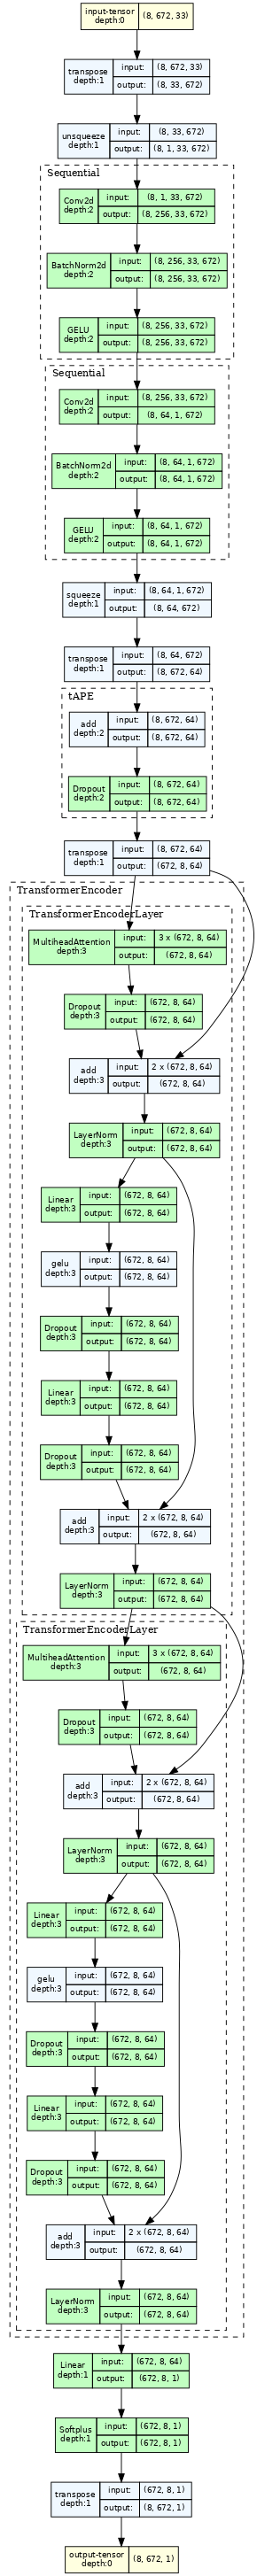
\includegraphics[height=\textheight]{chapters/3_models/imgs/gab/transformerarchitecture.png}
	\caption{Transformer Based Model architecture visualization.}\label{fig:gabarchitecture}
\end{figure}

\subsection{Training}
The model was trained using the input format discussed earlier,
generating gaps artificially in the training dataset, while also ensuring the
creation of a gap mask.
This mask is an array of the same length as the input time series,
composed of two elements: 1 to indicate the gap timestamps and 0 for regular timestamps.
This allows obtaining only the predicted values within the gap,
which are used for evaluating the loss function.

In this case, a procedure for normalizing the area was applied to ensure that the
model learns the gap curve's behavior.
The L1Loss\cite{loss} function was employed as the loss function, and AdamW\cite{adamw} was used as the
optimizer with a learning rate ($\lambda$) set to 0.00001.
The learning rate is then adjusted during training using a cosine annealing scheduler\cite{scheduler1}\cite{scheduler2}
to provide optimal conditions for the model during this phase.

Additionally, a validation dataset was used to assess the model's
performance during training and to enable the
\textit{Early Stopping}\cite{es} and \textit{Save Best} procedures,
which were also implemented in this case.

%Il modello è stato allenato utilizzando il formato di input discusso in
%precedenza andando a creare buchi in modo artificiale nel dataset
%di training facendo attenzione a generare anche una maschera del buco: un
%array di lunghezza pari a quella della serie passata in input e coposto da due elementi, 1 indica i timestamp del buco mentre 0 quelli ordinari.
%In questo modo sarà possibile andare ad ottenere solo i valori del buco
%predetti dal modello per poi valutare la loss function solo su questi valori.
%Anche in questo caso è stata applicata una procedura di normalizzazione dell'area
%per assicurarci che il modello impari ad apprendere l'andamendo della curva
%del buco. E' stata impiegata la L1Loss come loss function, AdamW come
%optimizer con learning rate $\lambda$ pari a 0.00001 che poi 
%verrà variato durante la procedura di training tramite un cosine annealing scheduler per permettere al modello le migliori condizioni durante questa
%fase.
%Anche in questo caso è stato impiegato il dataset di validation per andare
%a misurare le performance del modello durante l'allenamento e per permettere
%il funzionamento delle procedure 
%\textit{Early Stopping} e \textit{Save Bast} che anche inquesto caso 
%sono state implementate.

\begin{table}[H]
	\begin{center}
		\begin{tabular}[c]{l|l}
			\textbf{Total Parameters (\#)}     & 594177 \\
			\textbf{Trainable Parameters (\#)} & 594177 \\
			\textbf{Training Duration (s)}     & 900.0  \\
			\textbf{Model Size (MB)}           & 2.4
		\end{tabular}
	\end{center}
	\caption{Transformer based model specification.}\label{tab:gabspecs}
\end{table}

\begin{figure}[H]
	\centering
	\begin{tikzpicture}
		\draw[->] (-3,0) -- (3,0) node[right] {$x$};
		\draw[->] (0,-1) -- (0,2) node[above] {$y$};
		\draw[dotted] (-3,-1) grid (3,2);
		\draw[color=blue, domain=-3:2] plot[id=logistic] function{0.5 * x * (1+tanh(sqrt(2/pi) * (x + 0.044715*x**3)))};
	\end{tikzpicture}
	\caption{Gaussian Error Linear Units (GELU). $GELU(x) = x * \Phi(x)$}
	\label{fig:gelu}
\end{figure}

\begin{figure}[H]
	\centering
	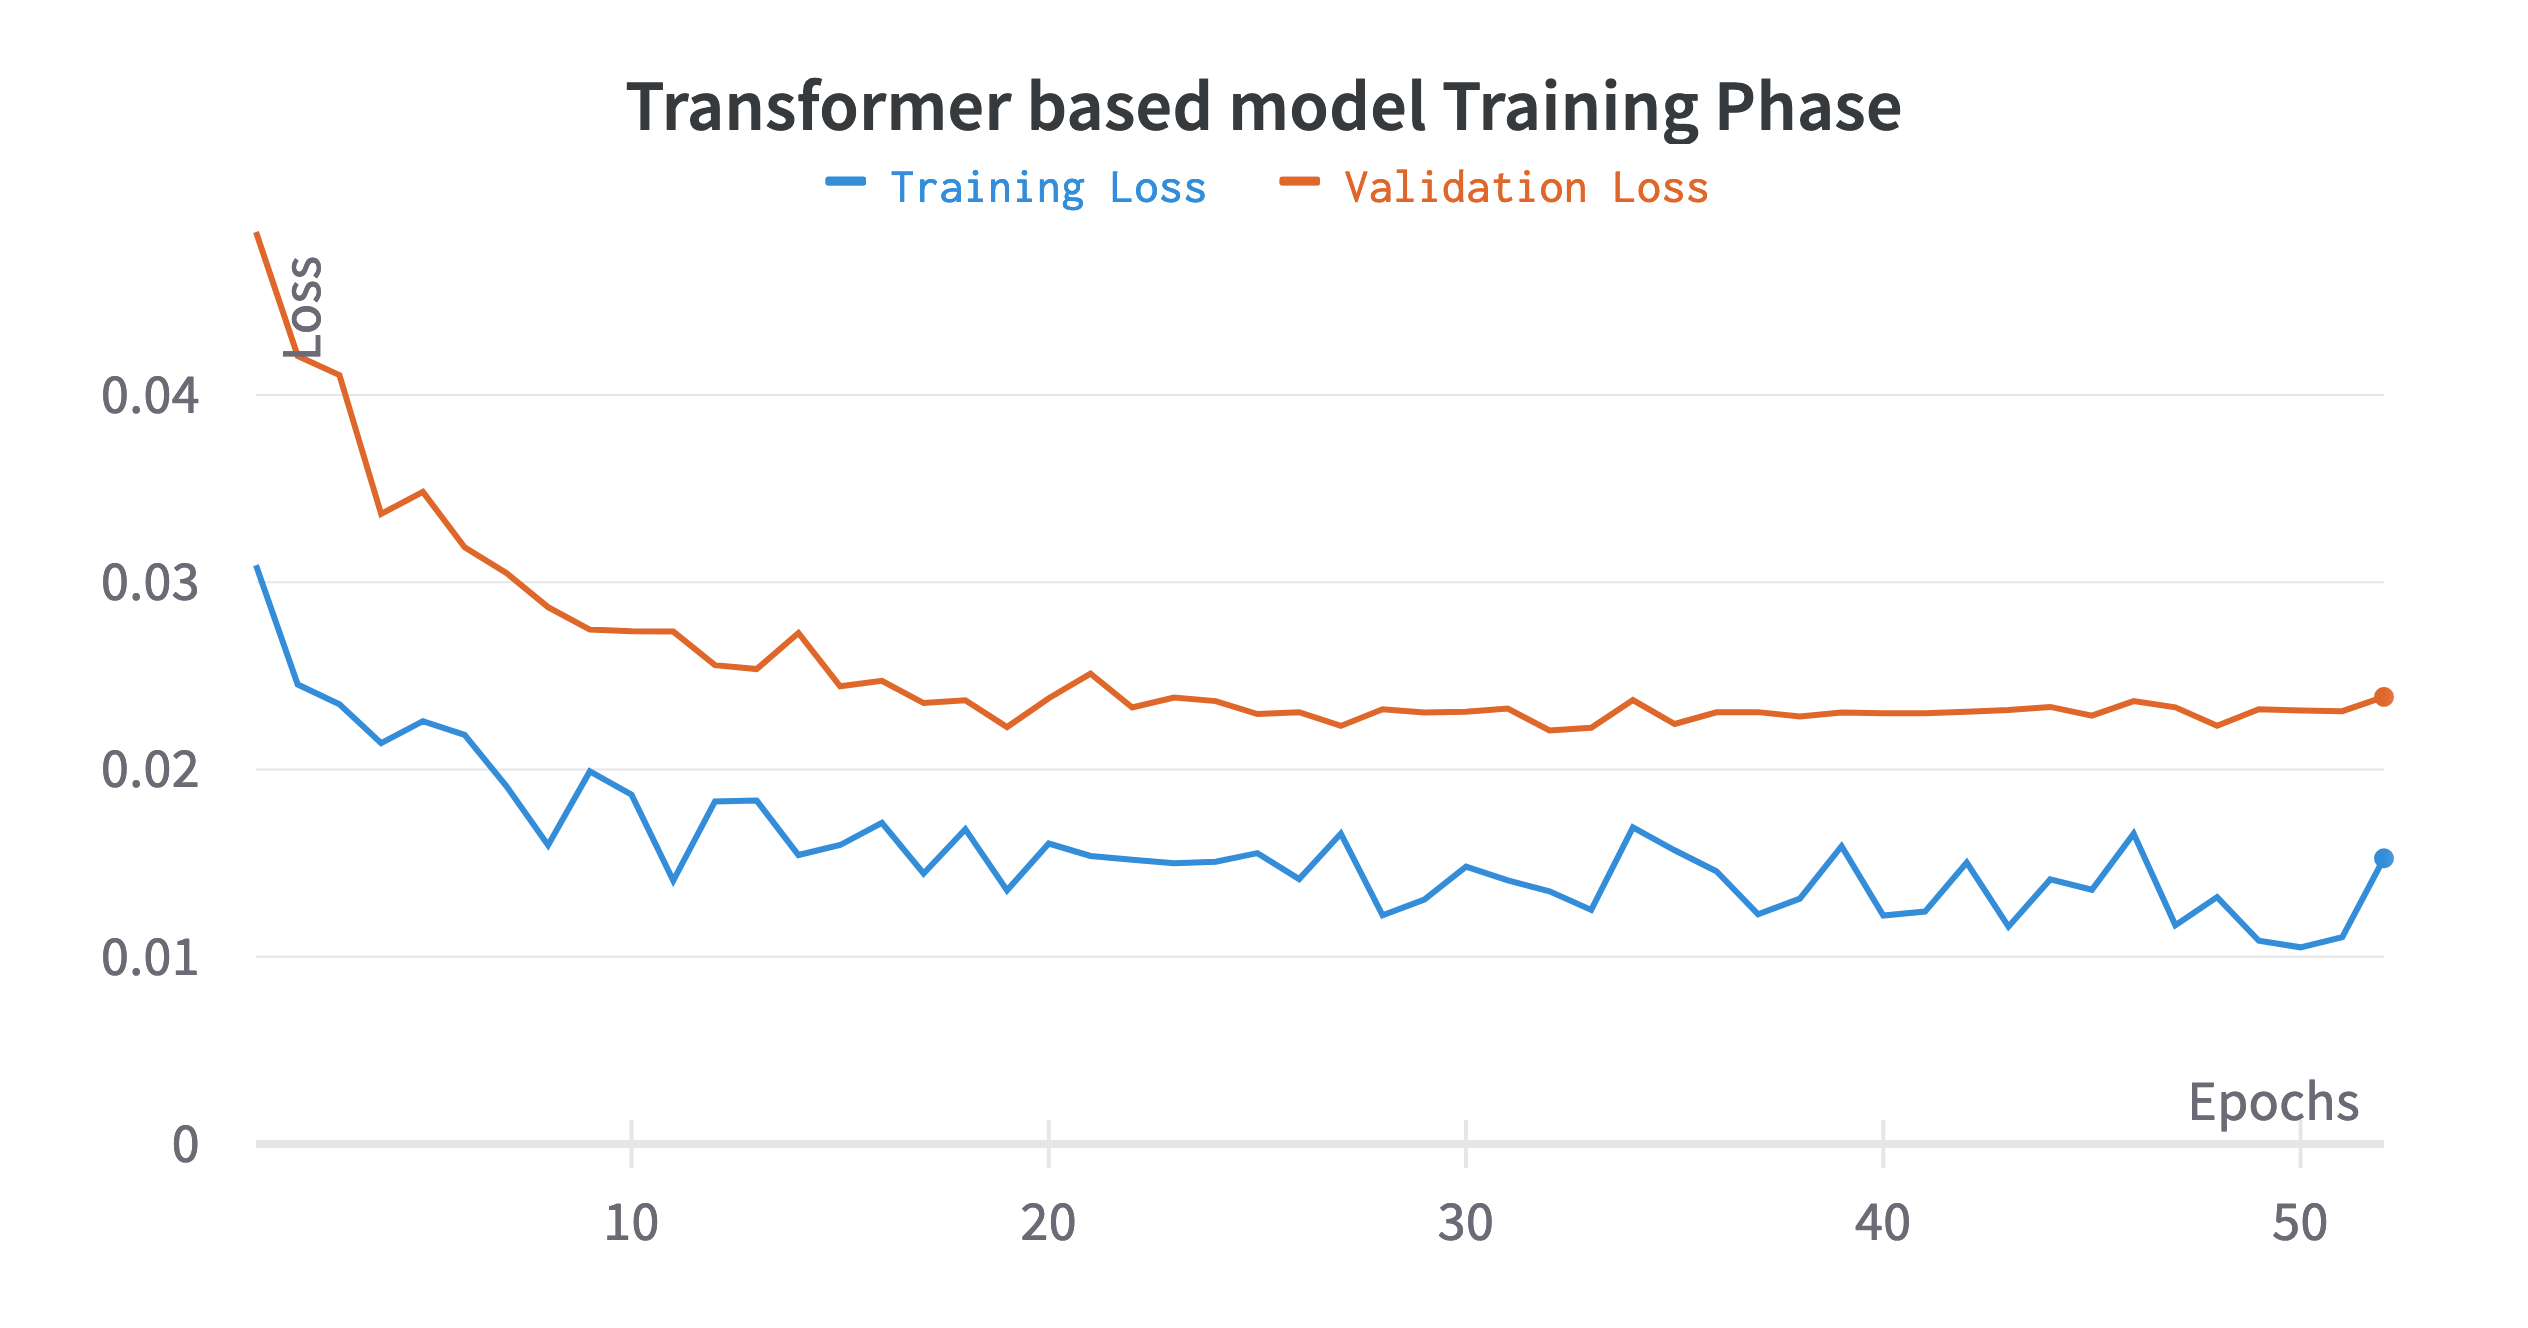
\includegraphics[width=.9\textwidth]{chapters/3_models/imgs/gab/gabtraining.png}
	\caption{The chart displays the loss progression during the training phase.The blue line represents the Training Loss, while the orange line represents the Validation Loss.}
	\label{fig:gabtrainchart}
\end{figure}

\begin{figure}[H]
	\centering
	\begin{subfigure}{0.43\textwidth}
		\centering
		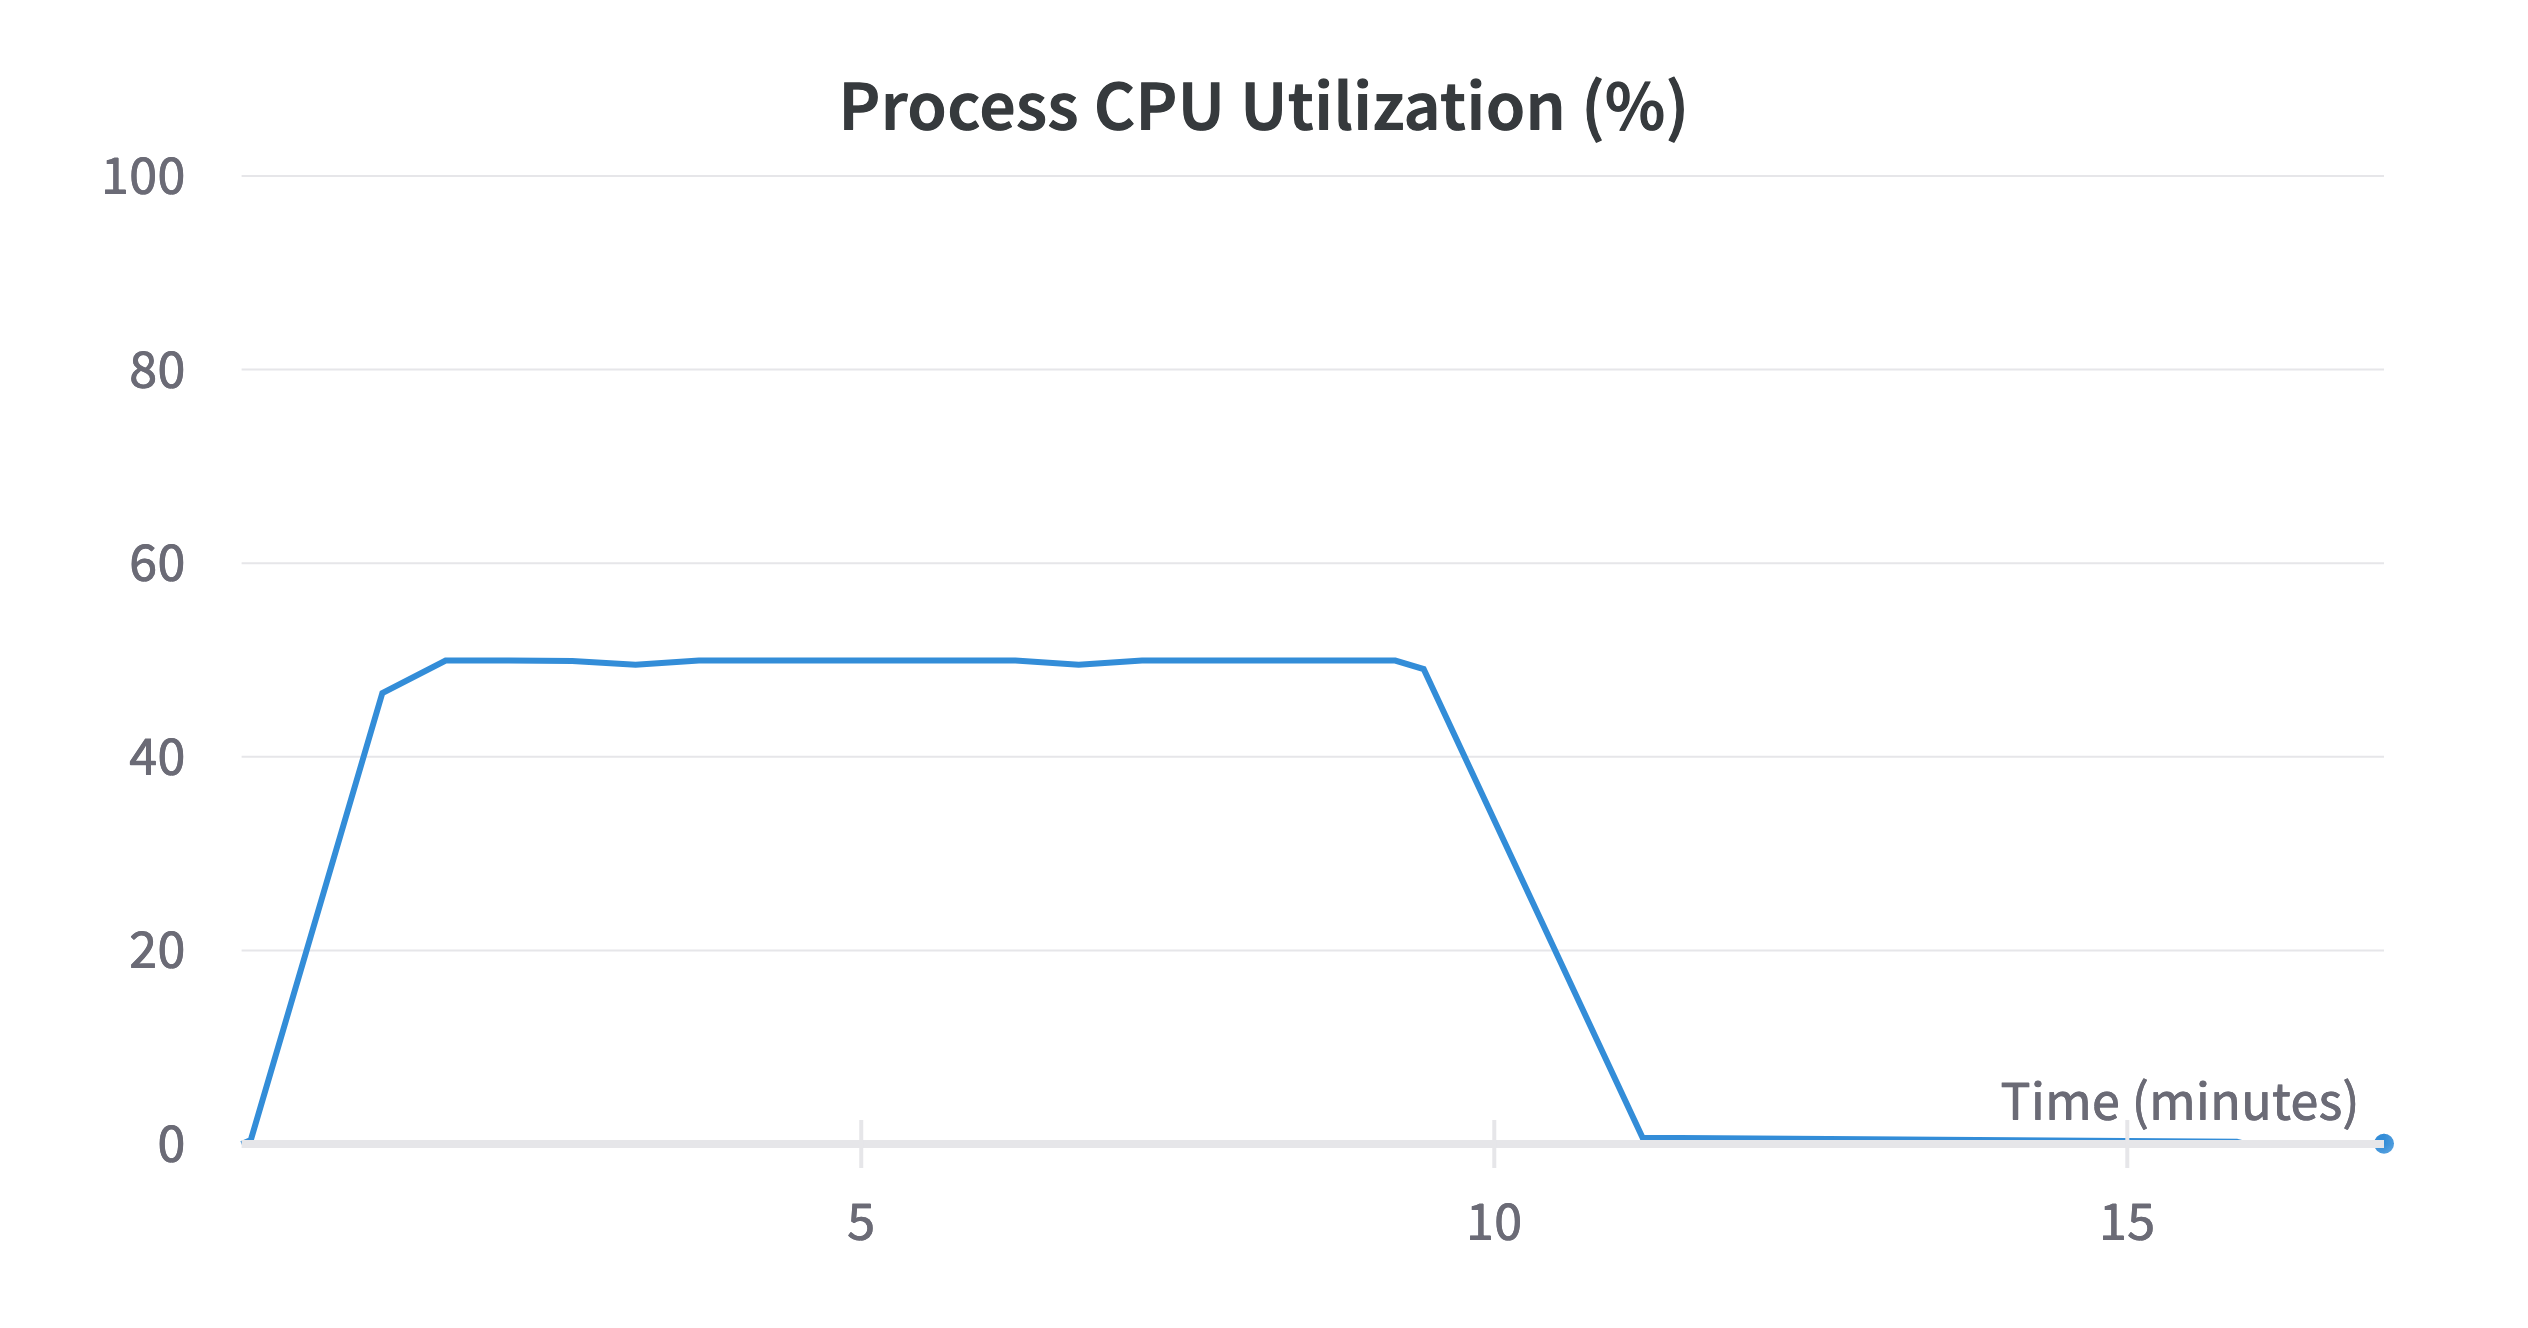
\includegraphics[width=\textwidth]{chapters/3_models/imgs/gab/train/gabrielcputilization.png}
	\end{subfigure}
	\begin{subfigure}{0.43\textwidth}
		\centering
		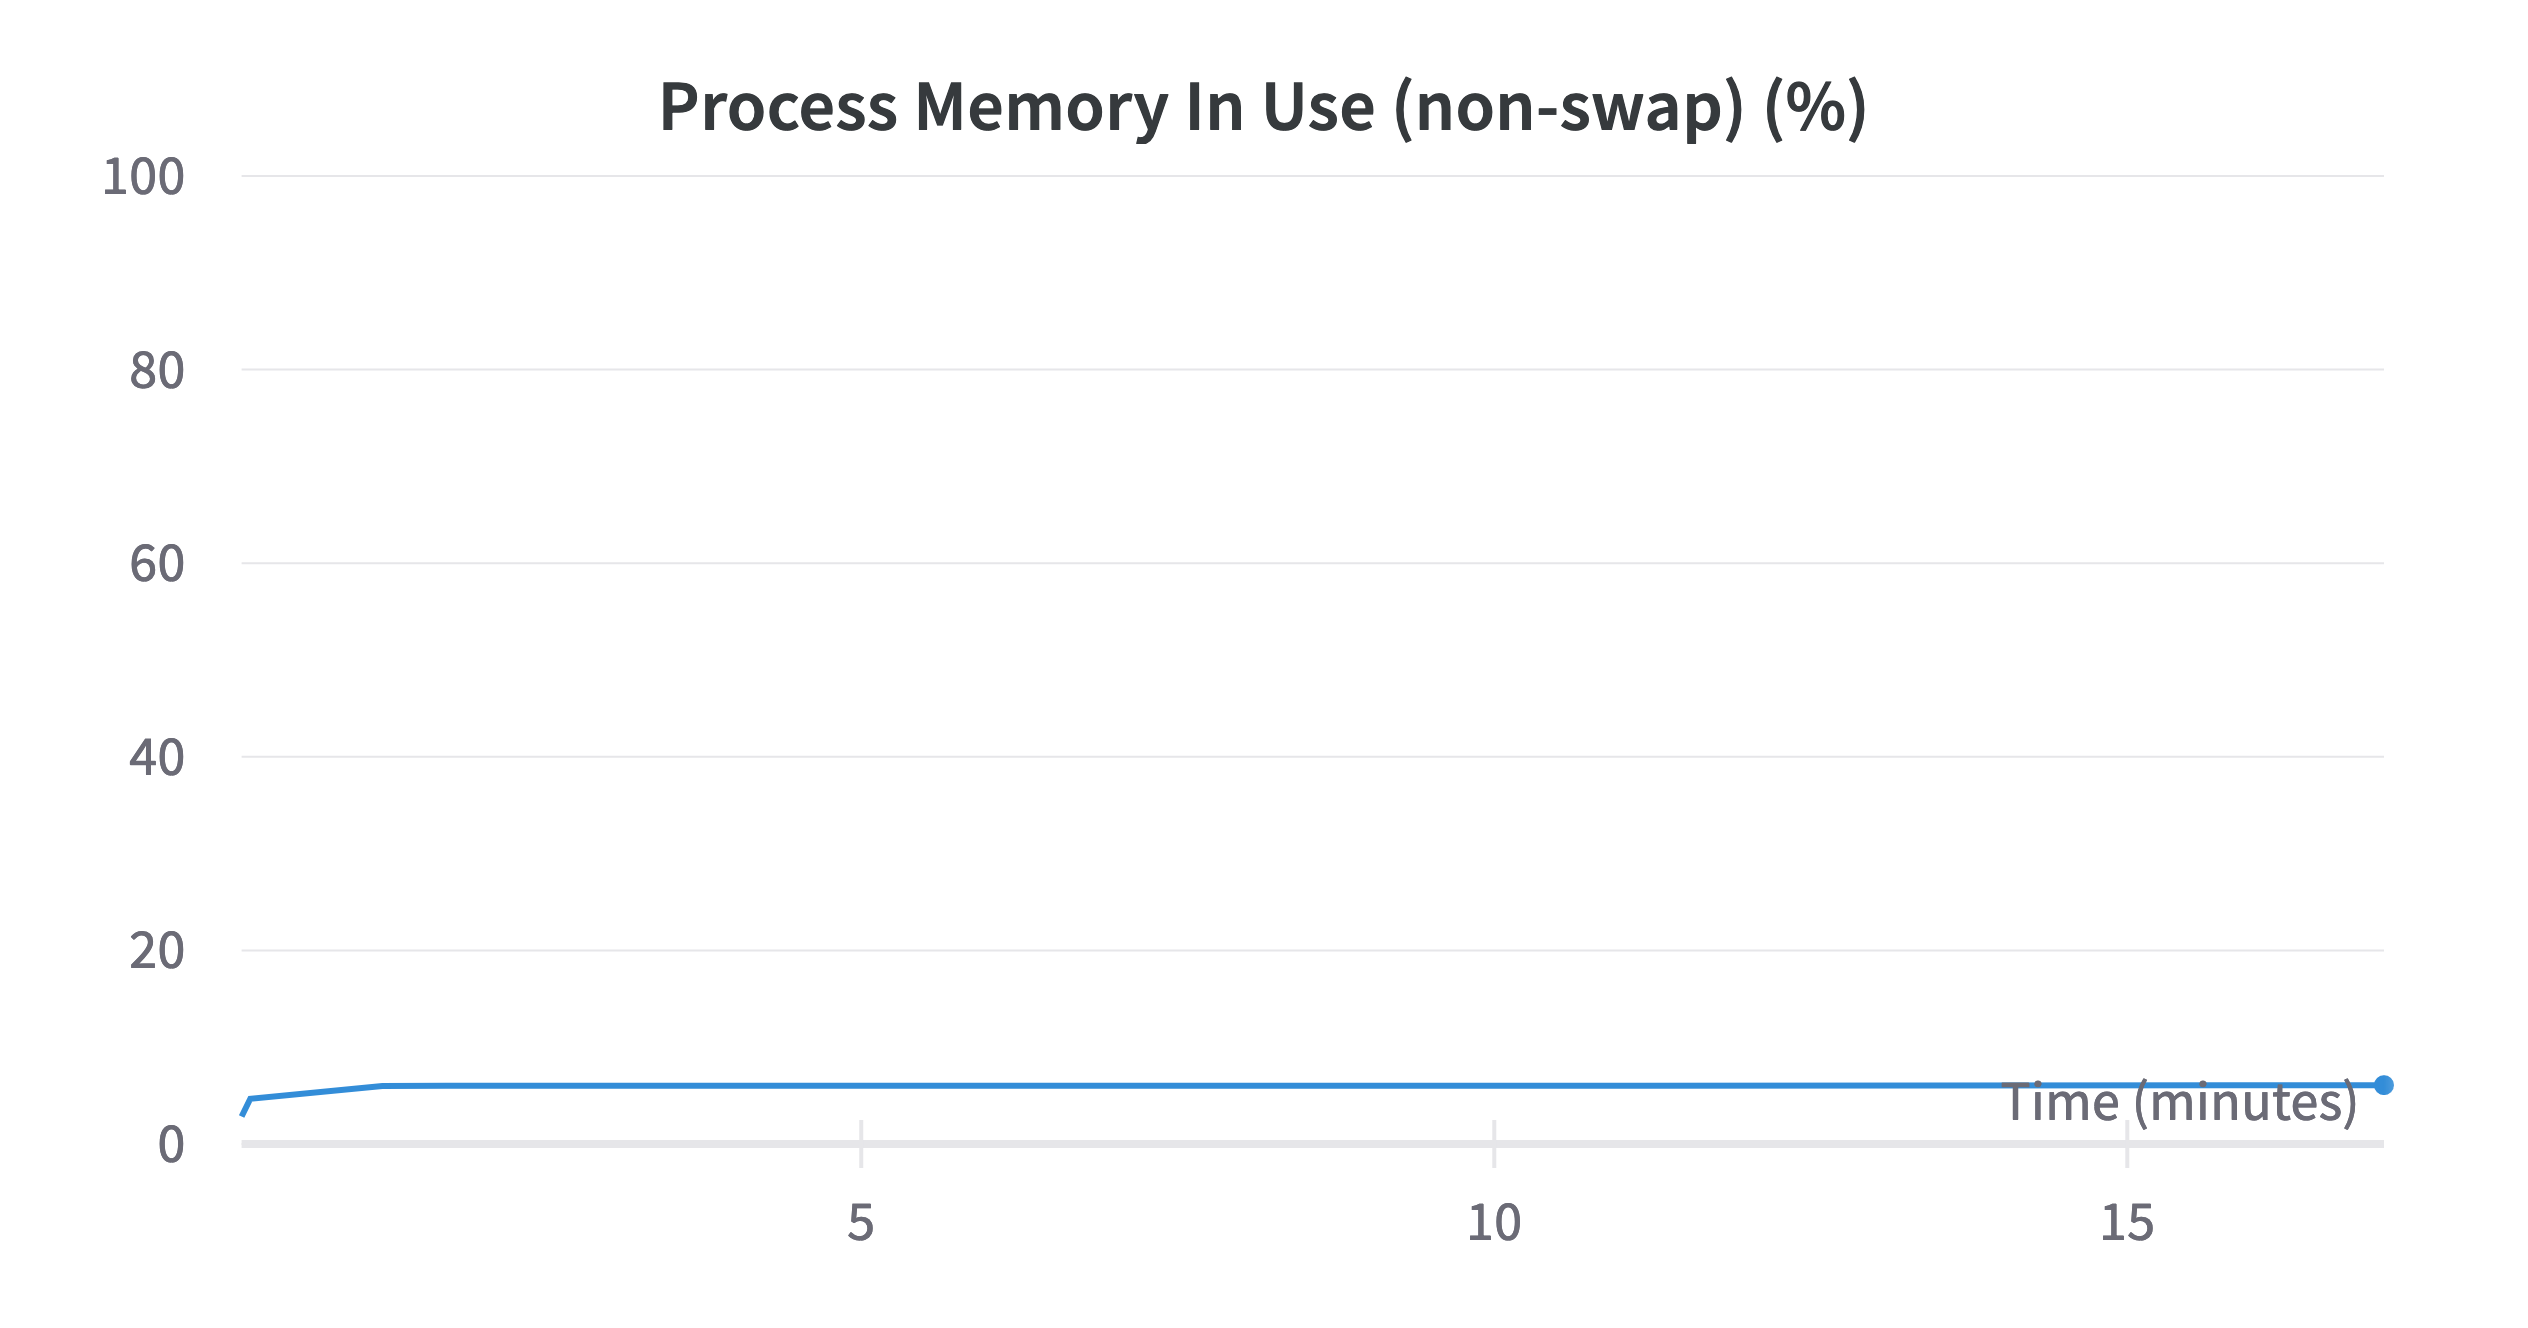
\includegraphics[width=\textwidth]{chapters/3_models/imgs/gab/train/gabrielprocessmemory.png}
	\end{subfigure}\\
	\begin{subfigure}{0.43\textwidth}
		\centering
		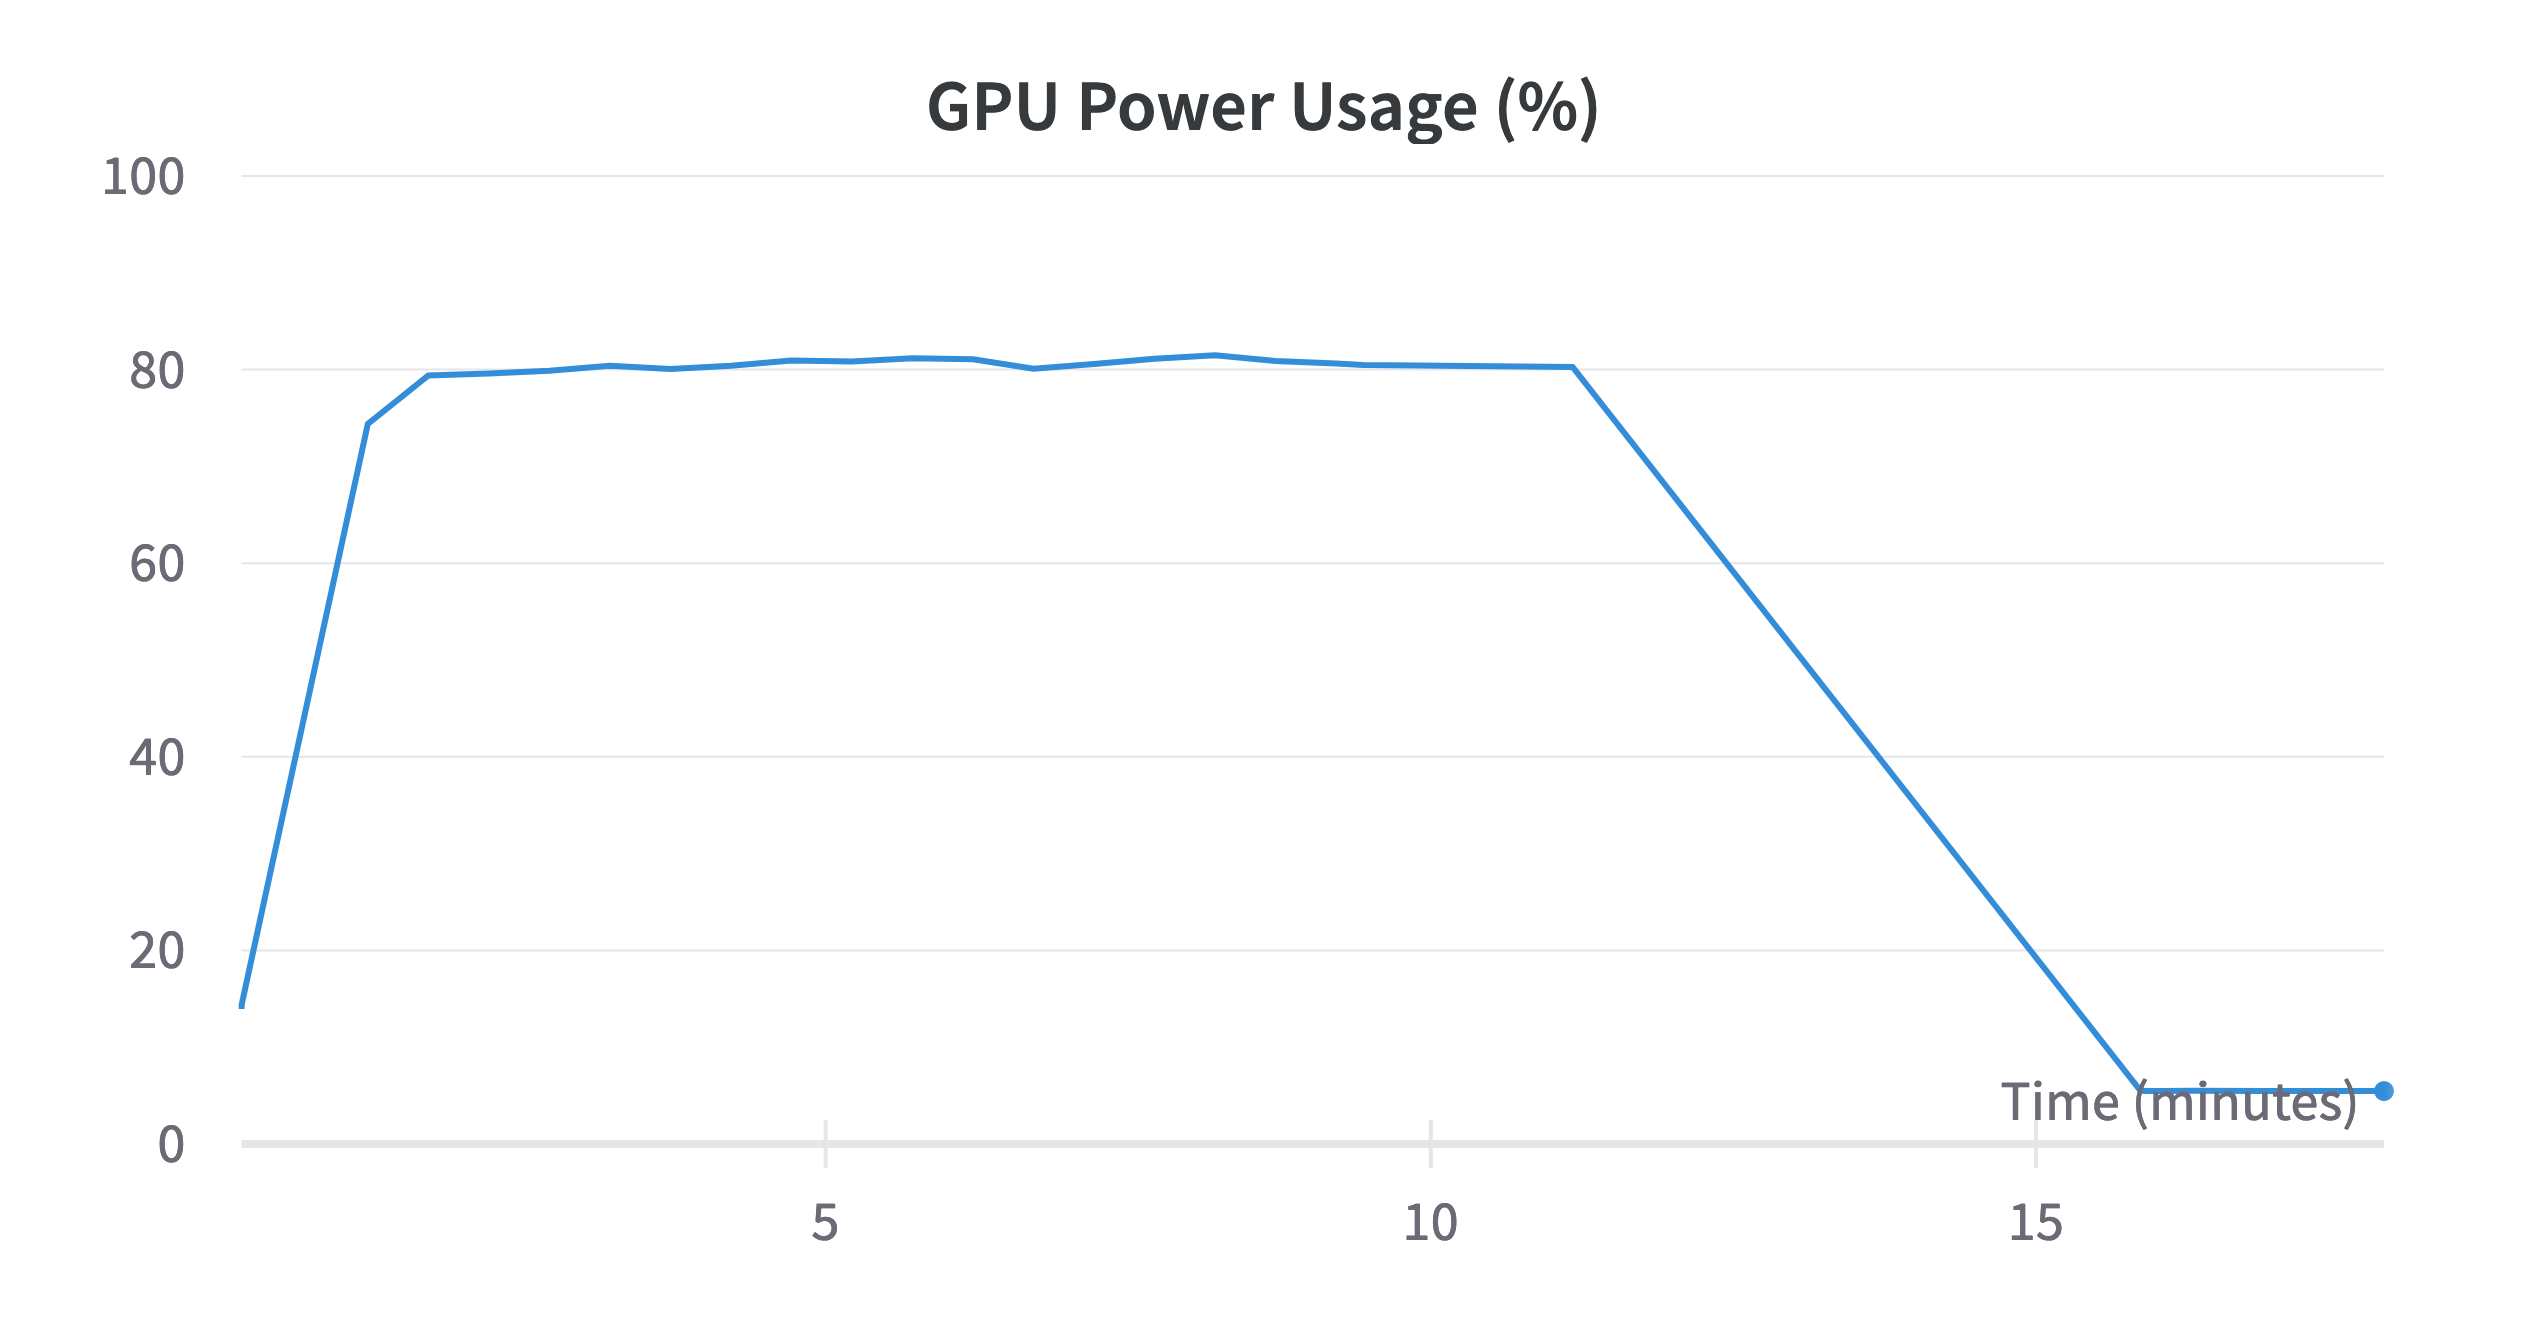
\includegraphics[width=\textwidth]{chapters/3_models/imgs/gab/train/gabrielgpupowerusageperc.png}
	\end{subfigure}
	\begin{subfigure}{0.43\textwidth}
		\centering
		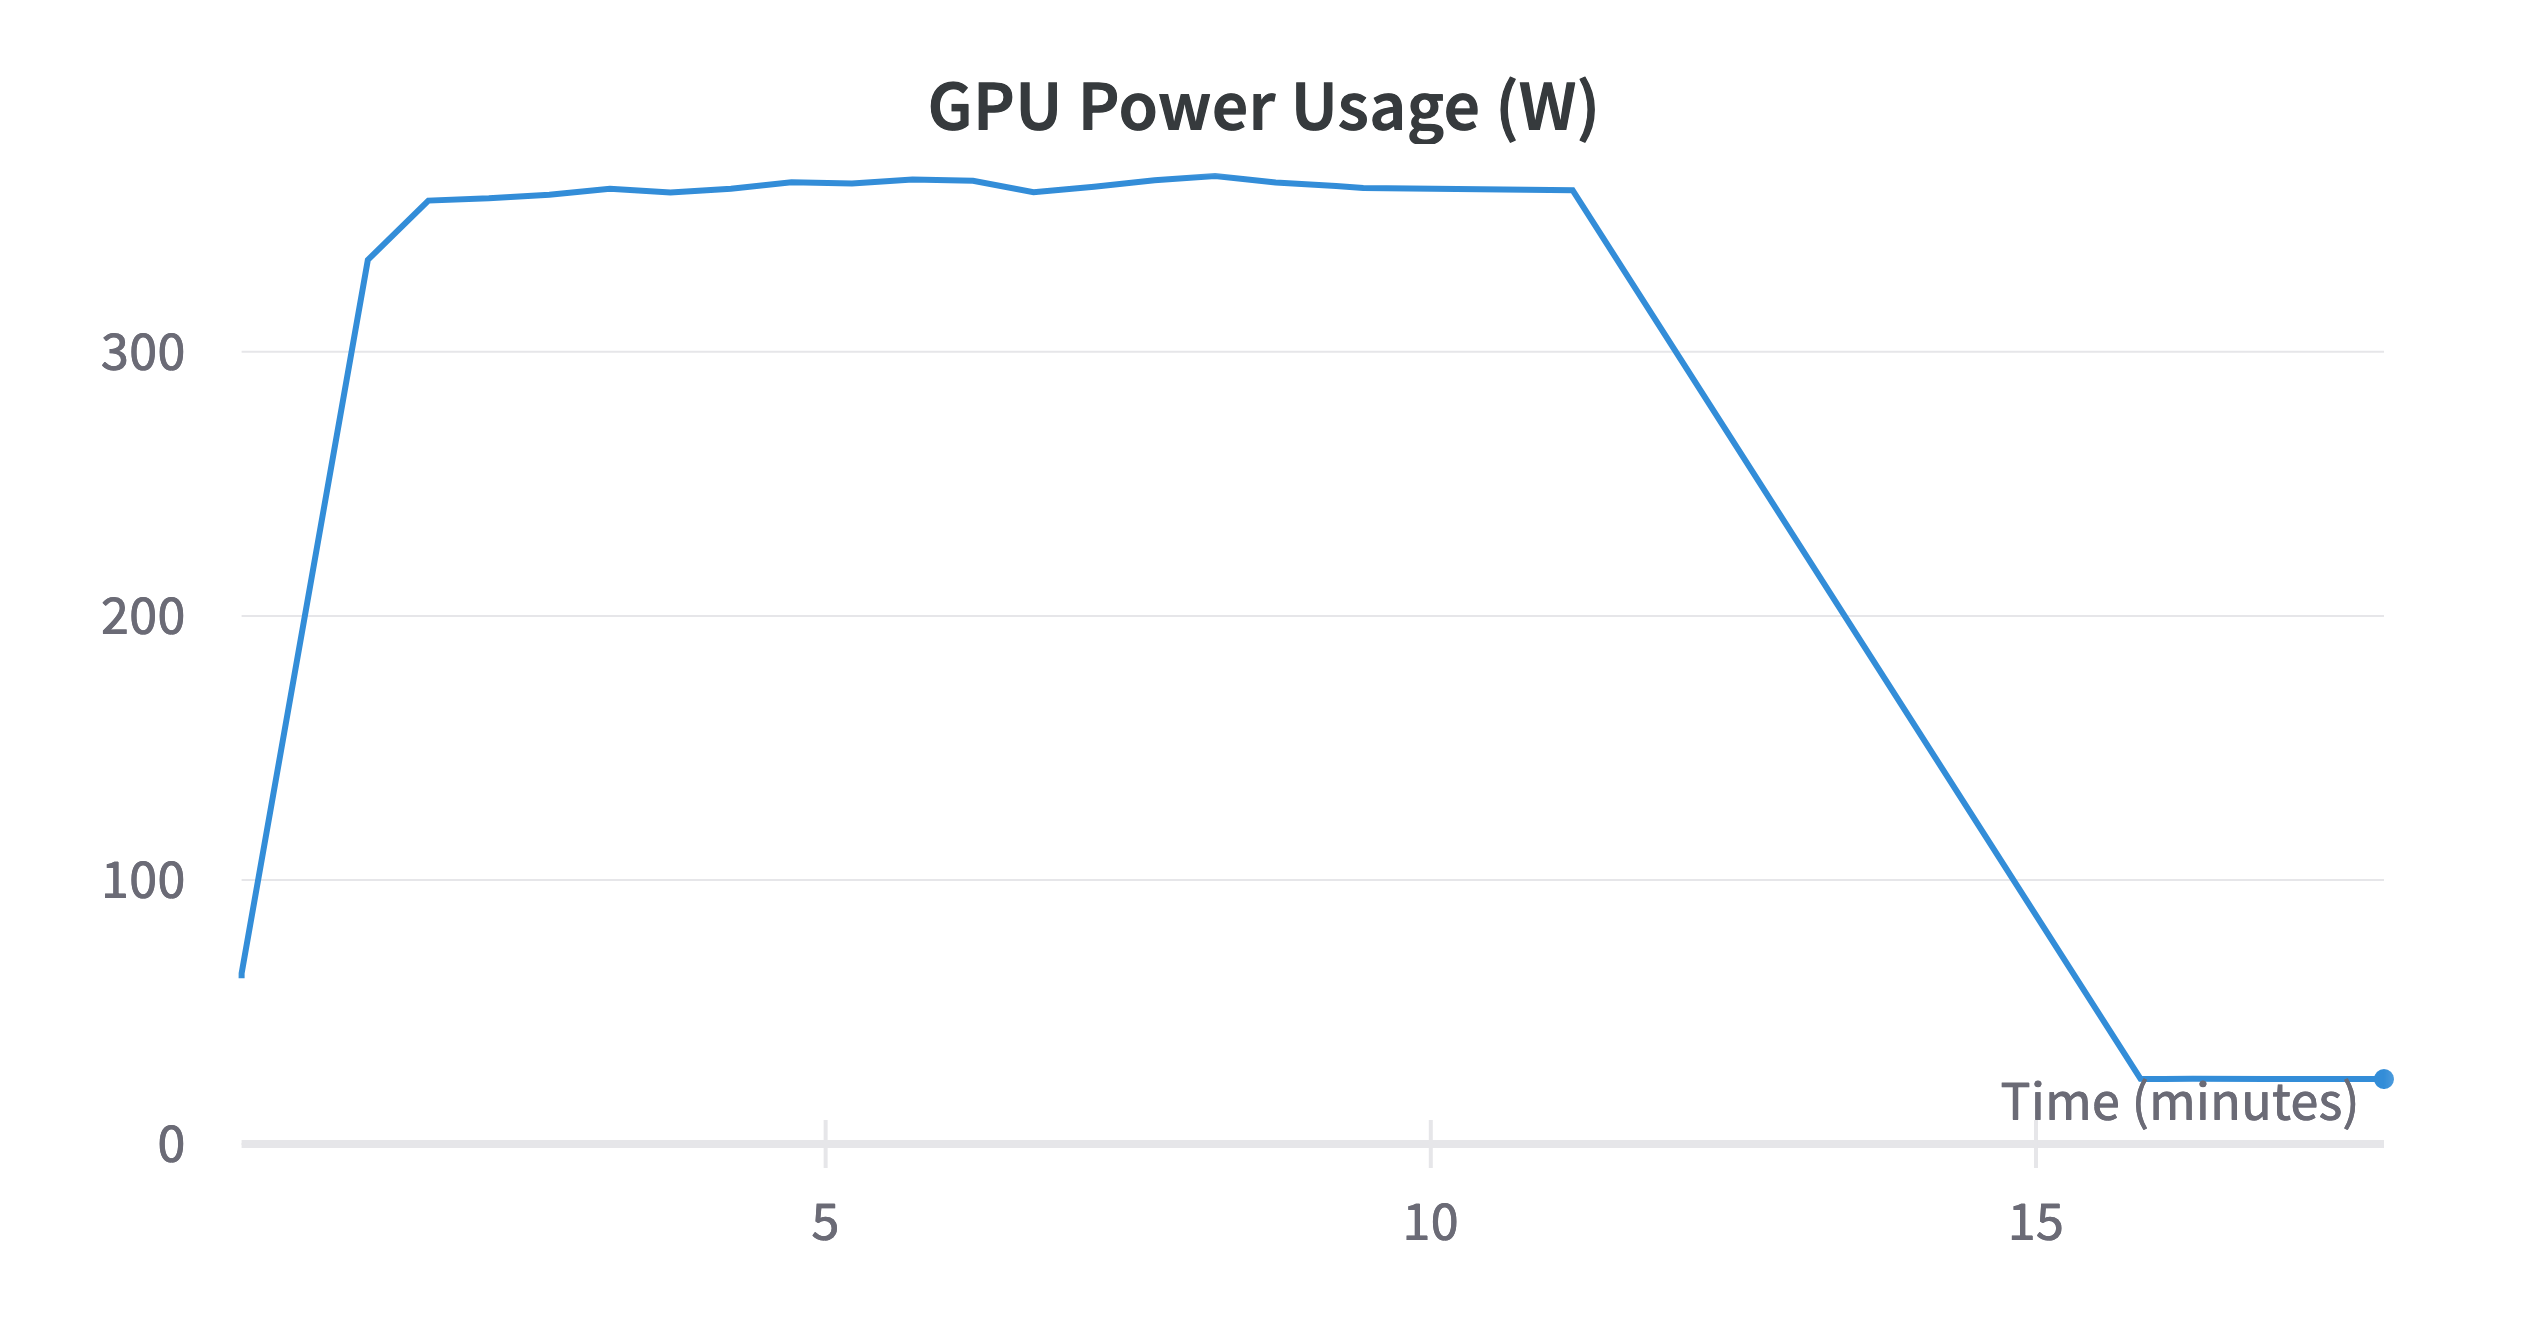
\includegraphics[width=\textwidth]{chapters/3_models/imgs/gab/train/gabrielgpupowerusagew.png}
	\end{subfigure}\\
	\begin{subfigure}{0.43\textwidth}
		\centering
		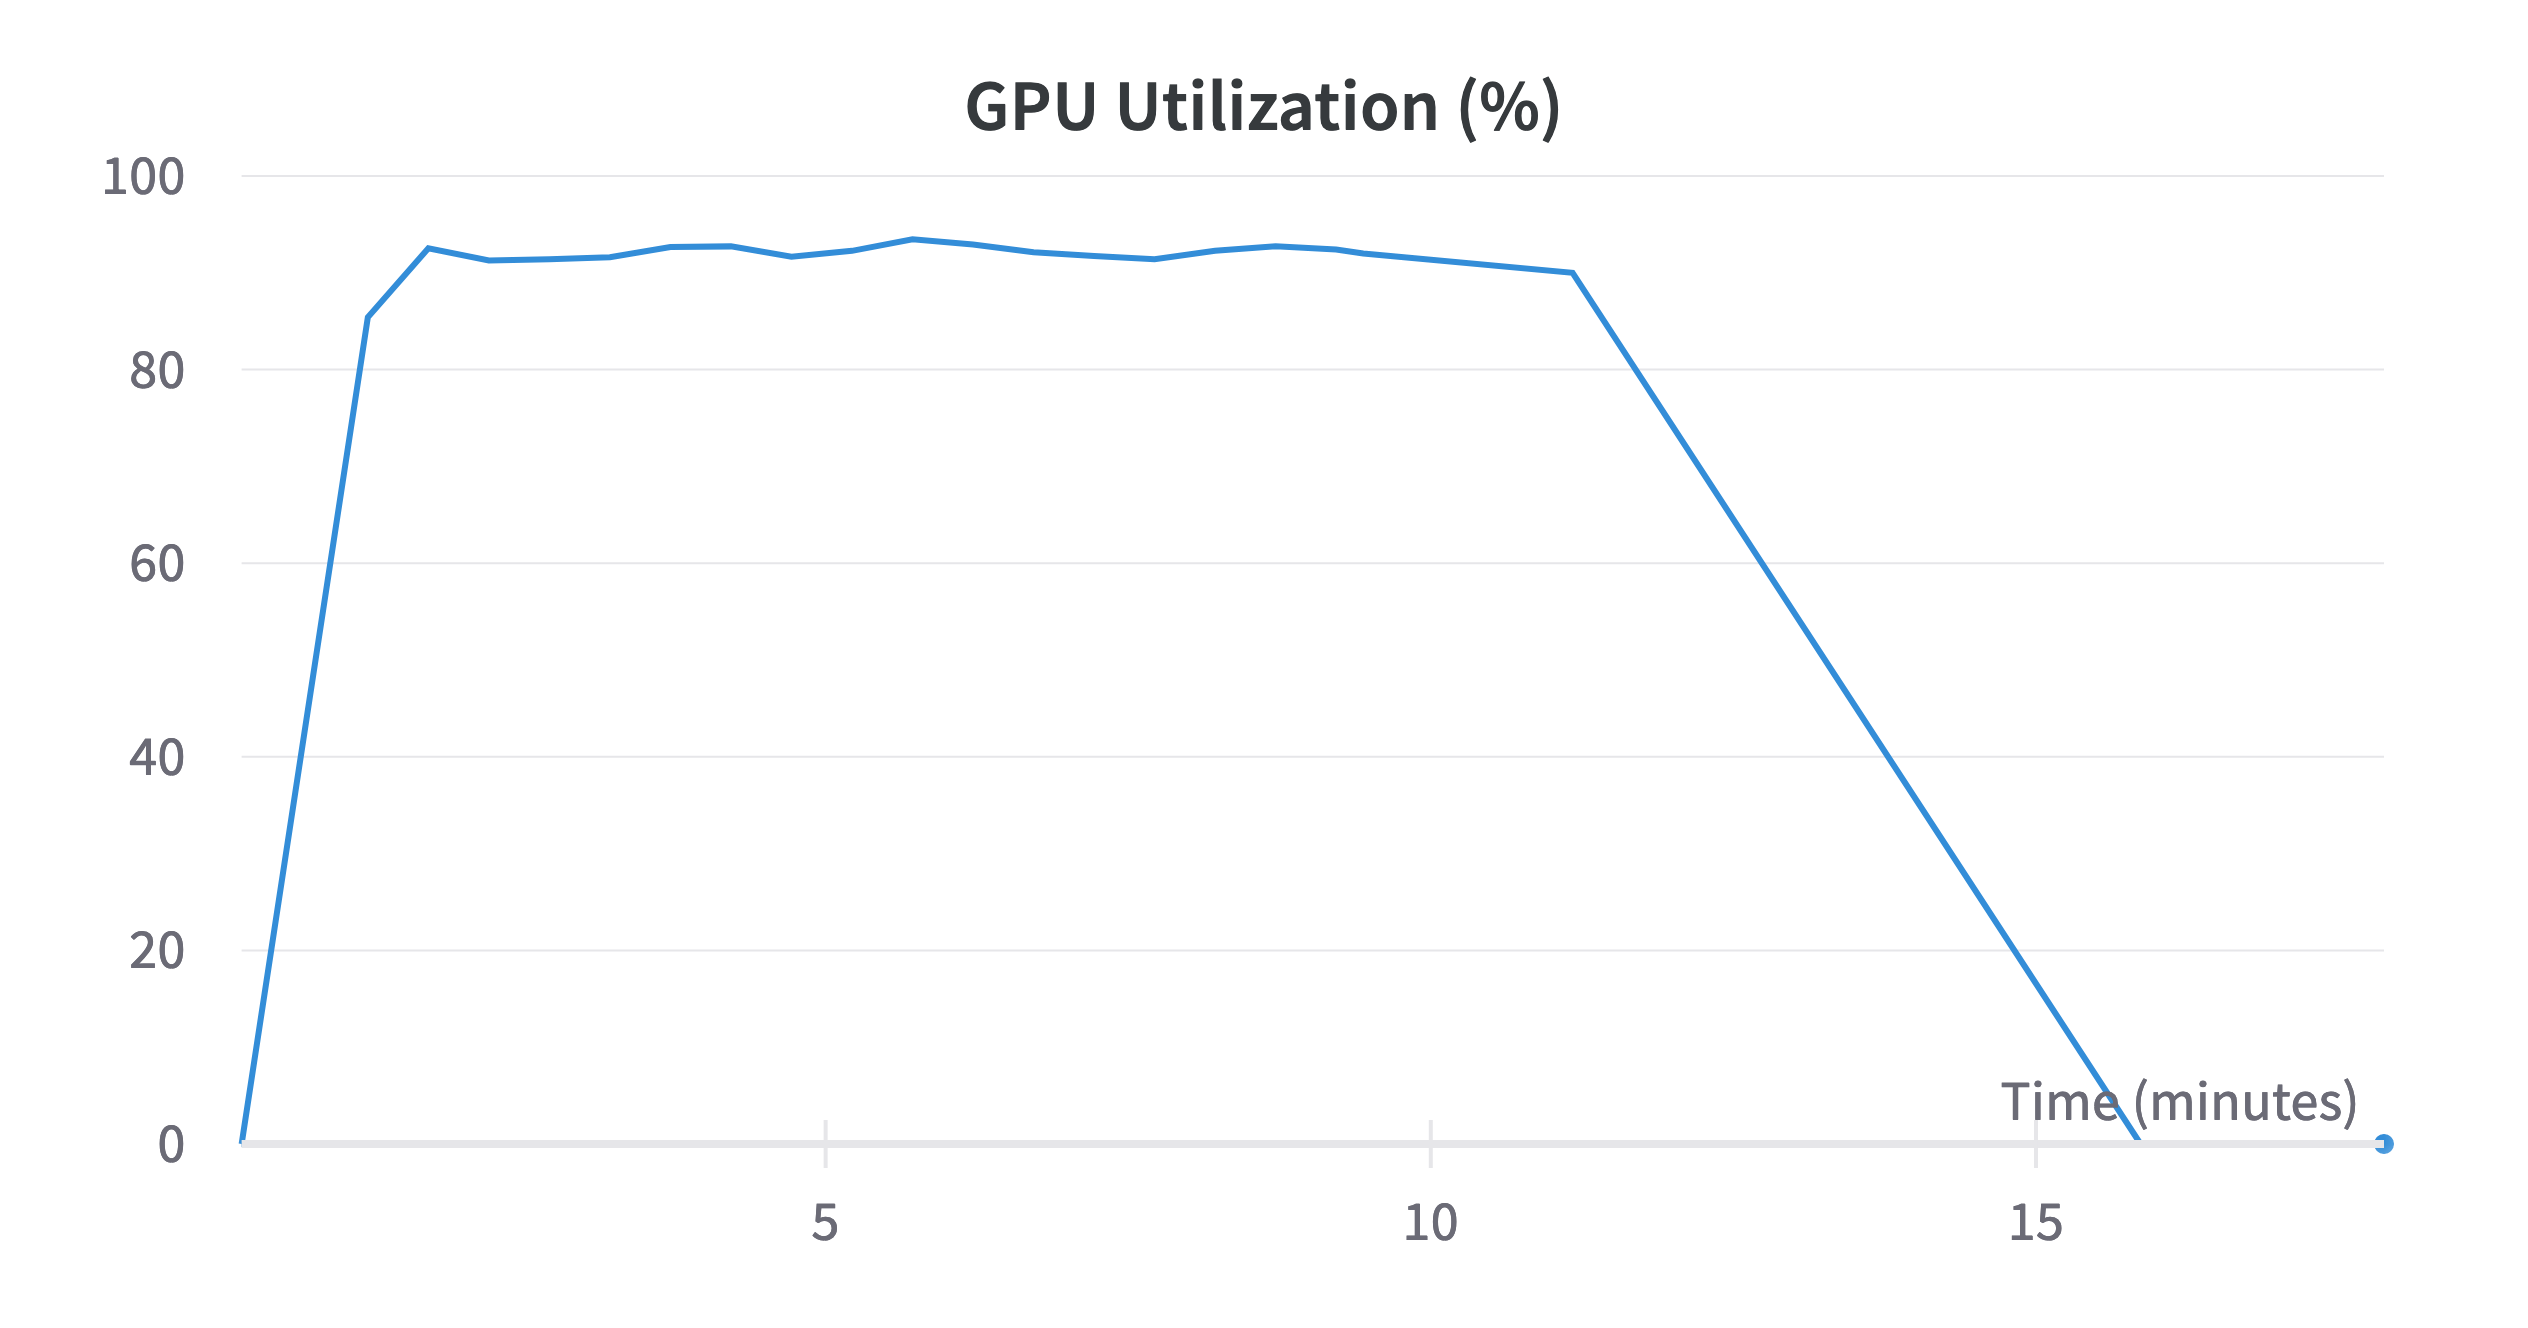
\includegraphics[width=\textwidth]{chapters/3_models/imgs/gab/train/gabrielgpuutilizationperc.png}
	\end{subfigure}
	\begin{subfigure}{0.43\textwidth}
		\centering
		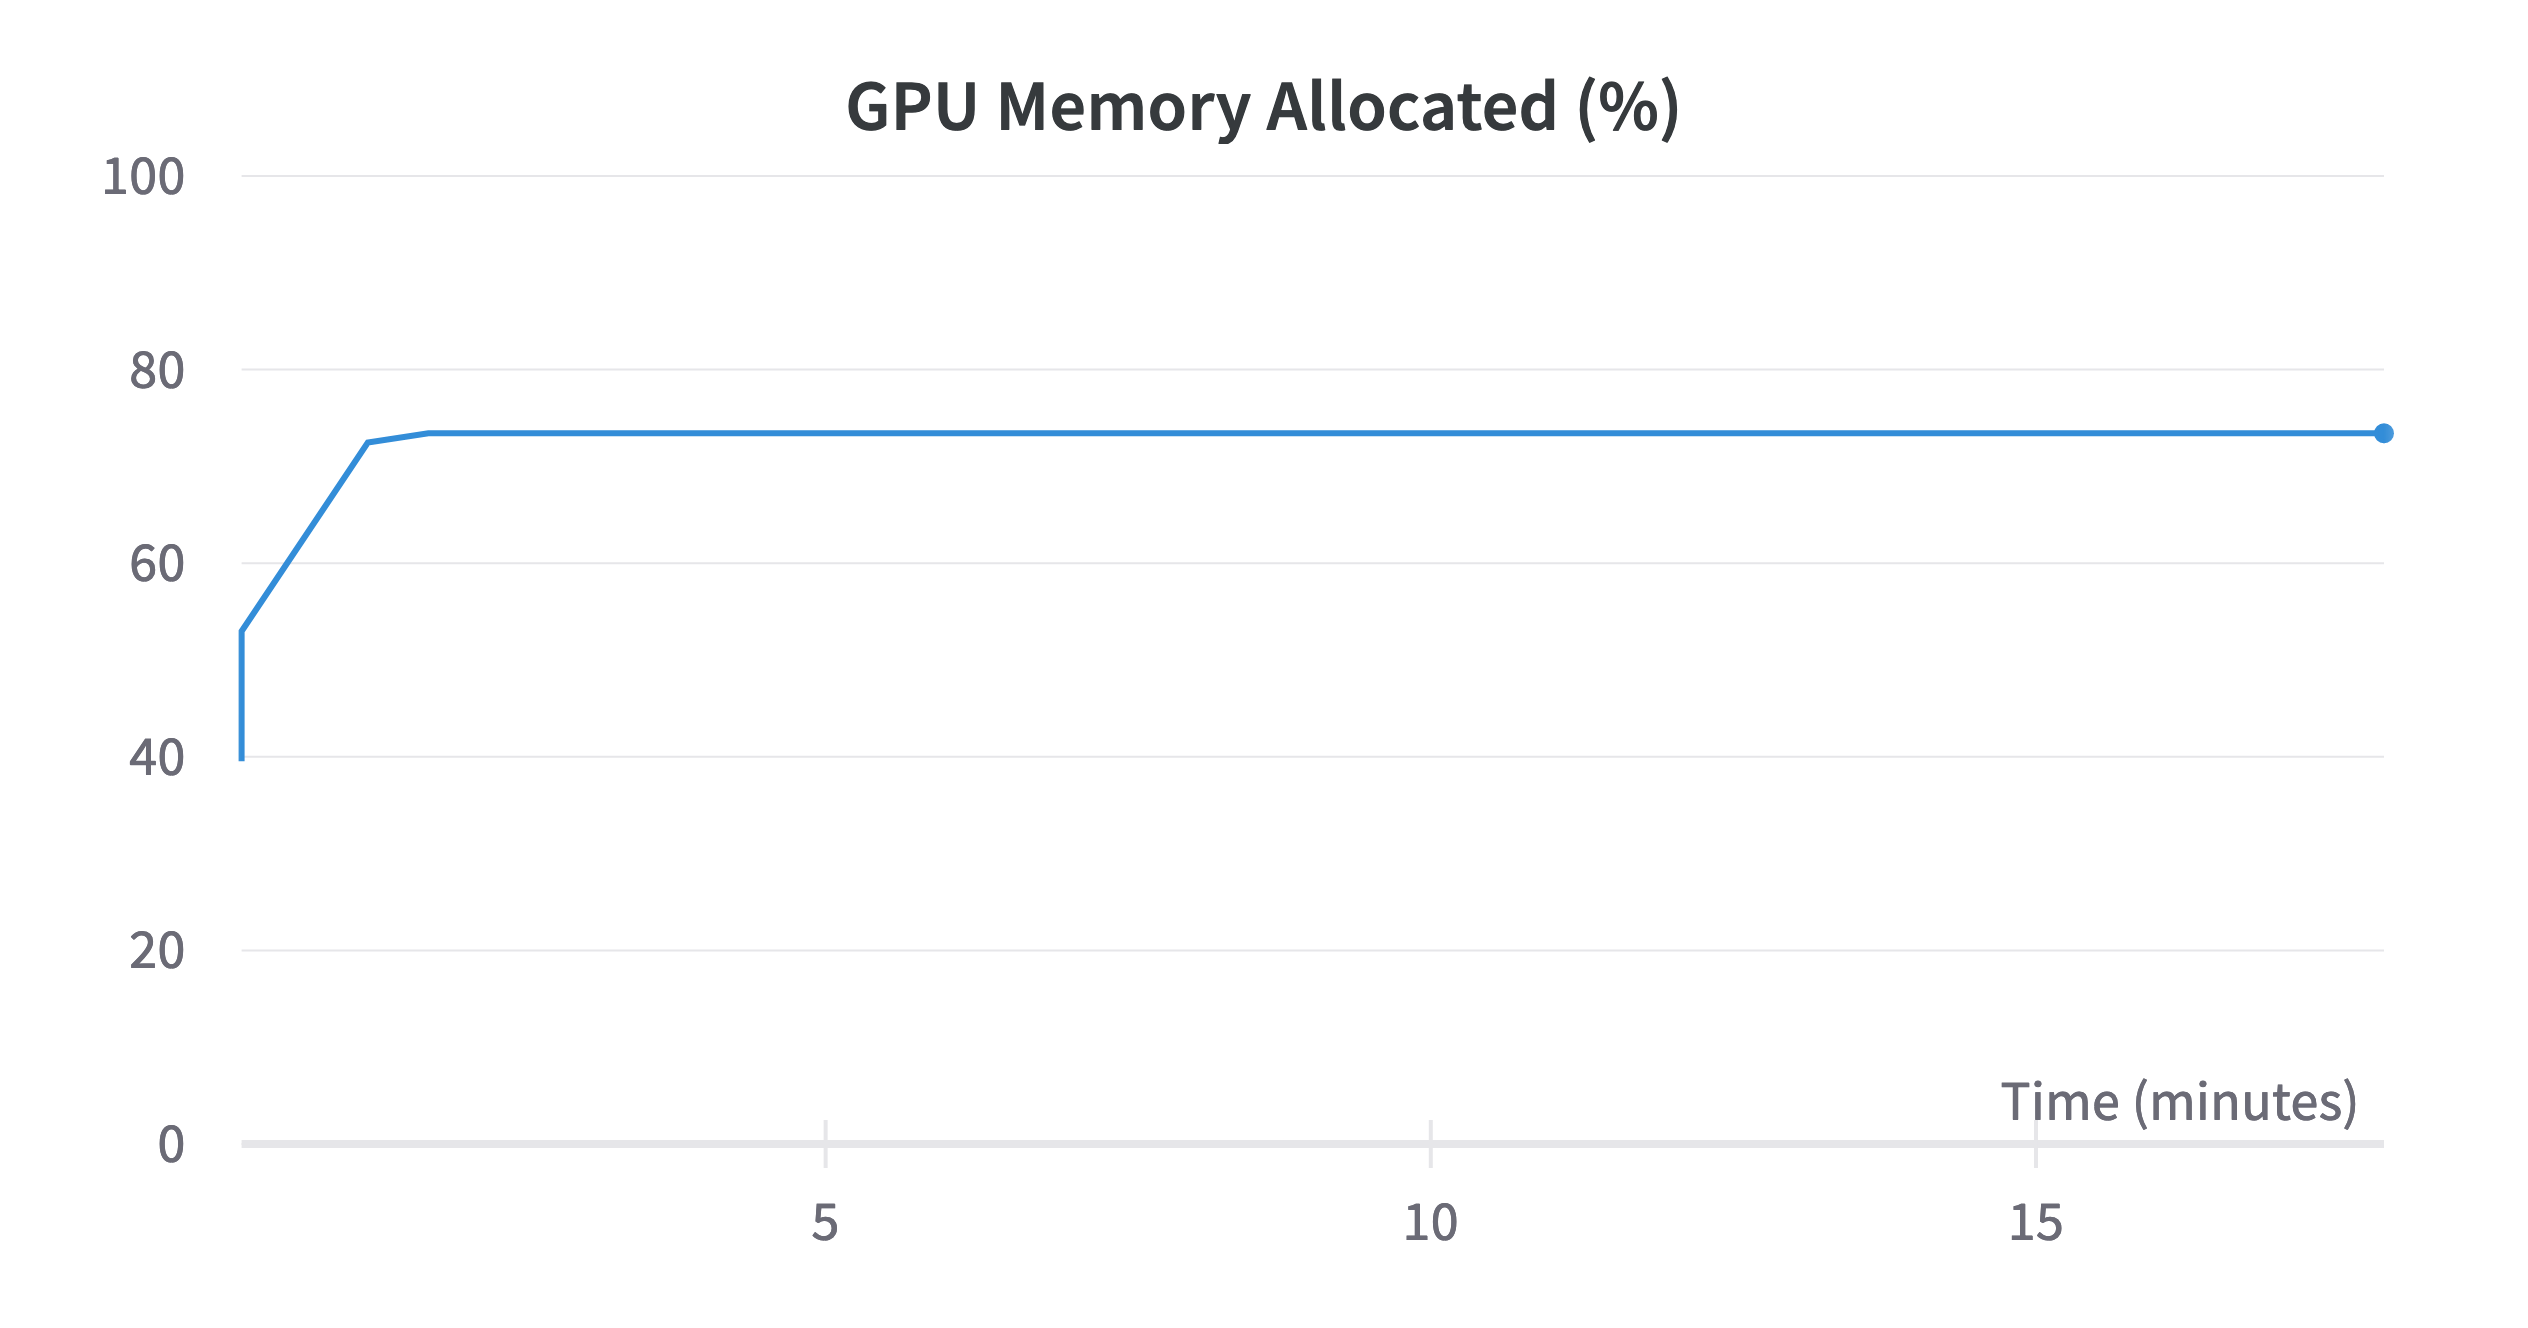
\includegraphics[width=\textwidth]{chapters/3_models/imgs/gab/train/gabrielgpumemalloc.png}
	\end{subfigure}\\
	\caption{System resources utilized during the Training phase.}
	\label{fig:gabsysusage}
\end{figure}


\begin{algorithm}[H]
	\caption{Transformer based model Training Algorithm}\label{alg:gabtraining}
	\begin{algorithmic}
		\Require train/validation datasets; Transformer based Neural Network Model

		\State Batch Size $\gets$ 8
		\State Learning Rate $\lambda \gets$ 0.00001
		\State Epochs $\gets$ 100
		\State Patience $\gets$ 20
		\State loss $\gets$ L1Loss()
		\State Optimizer $\gets$ AdamW Optimizer
		\State Scheduler $\gets$ CosineAnnealingScheduler
		\State Min Gap size $\gets$ 2 timestamps
		\State Max Gap size $\gets$ $\frac{\text{week length}}{3}$ timestamps
		\State
		\For{\textbf{each} epoch \textbf{in} epochs}
		\For{\textbf{each} (batch\_id, src\_data, tgt\_data, mask) \textbf{in} train.next\_batch()}

		\State train\_prediction $\gets$ model(src\_data) \Comment{Model inference}
		\State train\_prediction $\gets$ train\_prediction $\cdot$ mask
		\State train\_prediction $\gets \frac{\text{train\_prediction} \cdot \sum\text{train\_prediction}}{\sum tgt\_data}$ \Comment{Area normalization}
		\State train\_loss $\gets$ loss(train\_prediction[mask = 1], tgt\_data[mask = 1])
		\State Optimizer step
		\State Back Propagation
		\EndFor
		\State Scheduler step
		\State stop computing gradient
		\For{\textbf{each} (batch\_id, vs, vt, vm) \textbf{in} validation.next\_batch()}
		\State val\_prediction $\gets$ model(vs) \Comment{Model inference}
		\State val\_prediction $\gets$ val\_prediction $\cdot$ vm
		\State val\_prediction $\gets \frac{\text{val\_prediction} \cdot \sum\text{val\_prediction}}{\sum vt}$ \Comment{Area normalization}
		\State val\_loss $\gets$ loss(val\_prediction[vm = 1], vt[vm = 1])
		\EndFor

		\State check for Early Stopping
		\State check for Save Best Result
		\State start computing gradient
		\EndFor
	\end{algorithmic}
\end{algorithm}
